\documentclass[a4paper]{article}

\input{style/ch_xelatex.tex}
\input{style/scala.tex}

%代码段设置
\lstset{numbers=left,
basicstyle=\tiny,
numberstyle=\tiny,
keywordstyle=\color{blue!70},
commentstyle=\color{red!50!green!50!blue!50},
frame=single, rulesepcolor=\color{red!20!green!20!blue!20},
escapeinside=``
}

\graphicspath{ {images/} }
\usepackage{ctex}
\usepackage{graphicx}
\usepackage{color,framed}%文本框
\usepackage{listings}
\usepackage{caption}
\usepackage{amssymb}
\usepackage{enumerate}
\usepackage{xcolor}
\usepackage{bm} 
\usepackage{lastpage}%获得总页数
\usepackage{fancyhdr}
\usepackage{tabularx}  
\usepackage{geometry}
\usepackage{minted}
\usepackage{graphics}
\usepackage{subfigure}
\usepackage{float}
\usepackage{pdfpages}
\usepackage{pgfplots}
\pgfplotsset{width=10cm,compat=1.9}
\usepackage{multirow}
\usepackage{footnote}
\usepackage{booktabs}

%-----------------------伪代码------------------
\usepackage{algorithm}  
\usepackage{algorithmicx}  
\usepackage{algpseudocode}  
\floatname{algorithm}{Algorithm}  
\renewcommand{\algorithmicrequire}{\textbf{Input:}}  
\renewcommand{\algorithmicensure}{\textbf{Output:}} 
\usepackage{lipsum}  
\makeatletter
\newenvironment{breakablealgorithm}
  {% \begin{breakablealgorithm}
  \begin{center}
     \refstepcounter{algorithm}% New algorithm
     \hrule height.8pt depth0pt \kern2pt% \@fs@pre for \@fs@ruled
     \renewcommand{\caption}[2][\relax]{% Make a new \caption
      {\raggedright\textbf{\ALG@name~\thealgorithm} ##2\par}%
      \ifx\relax##1\relax % #1 is \relax
         \addcontentsline{loa}{algorithm}{\protect\numberline{\thealgorithm}##2}%
      \else % #1 is not \relax
         \addcontentsline{loa}{algorithm}{\protect\numberline{\thealgorithm}##1}%
      \fi
      \kern2pt\hrule\kern2pt
     }
  }{% \end{breakablealgorithm}
     \kern2pt\hrule\relax% \@fs@post for \@fs@ruled
  \end{center}
  }
\makeatother
%------------------------代码-------------------
\usepackage{xcolor} 
\usepackage{listings} 
\lstset{ 
breaklines,%自动换行
basicstyle=\small,
escapeinside=``,
keywordstyle=\color{ blue!70} \bfseries,
commentstyle=\color{red!50!green!50!blue!50},% 
stringstyle=\ttfamily,% 
extendedchars=false,% 
linewidth=\textwidth,% 
numbers=left,% 
numberstyle=\tiny \color{blue!50},% 
frame=trbl% 
rulesepcolor= \color{ red!20!green!20!blue!20} 
}

%-------------------------页面边距--------------
\geometry{a4paper,left=2.3cm,right=2.3cm,top=2.7cm,bottom=2.7cm}
%-------------------------页眉页脚--------------
\usepackage{fancyhdr}
\pagestyle{fancy}
\lhead{\kaishu \leftmark}
% \chead{}
\rhead{\kaishu 并行程序设计实验报告}%加粗\bfseries 
\lfoot{}
\cfoot{\thepage}
\rfoot{}
\renewcommand{\headrulewidth}{0.1pt}  
\renewcommand{\footrulewidth}{0pt}%去掉横线
\newcommand{\HRule}{\rule{\linewidth}{0.5mm}}%标题横线
\newcommand{\HRulegrossa}{\rule{\linewidth}{1.2mm}}
\setlength{\textfloatsep}{10mm}%设置图片的前后间距
%--------------------文档内容--------------------

\begin{document}
\renewcommand{\contentsname}{目\ 录}
\renewcommand{\appendixname}{附录}
\renewcommand{\appendixpagename}{附录}
\renewcommand{\refname}{参考文献} 
\renewcommand{\figurename}{图}
\renewcommand{\tablename}{表}
\renewcommand{\today}{\number\year 年 \number\month 月 \number\day 日}

%-------------------------封面----------------
\begin{titlepage}
    \begin{center}
    \includegraphics[width=0.8\textwidth]{NKU.png}\\[1cm]
    \vspace{20mm}
		\textbf{\huge\textbf{\kaishu{计算机学院}}}\\[0.5cm]
		\textbf{\huge{\kaishu{并行程序设计实验报告}}}\\[2.3cm]
		\textbf{\Huge\textbf{\kaishu{SIMD编程}}}

		\vspace{\fill}
    
    % \textbf{\Large \textbf{并行程序设计期末实验报告}}\\[0.8cm]
    % \HRule \\[0.9cm]
    % \HRule \\[2.0cm]
    \centering
    \textsc{\LARGE \kaishu{姓名\ :\ 仇科文}}\\[0.5cm]
    \textsc{\LARGE \kaishu{学号\ :\ 2312237}}\\[0.5cm]
    \textsc{\LARGE \kaishu{专业\ :\ 计算机科学与技术}}\\[0.5cm]
    
    \vfill
    {\Large \today}
    \end{center}
\end{titlepage}

\renewcommand {\thefigure}{\thesection{}.\arabic{figure}}%图片按章标号
\renewcommand{\figurename}{图}
\renewcommand{\contentsname}{目录}  
\cfoot{\thepage\ of \pageref{LastPage}}%当前页 of 总页数


% 生成目录
\clearpage
\tableofcontents
\newpage

\section{前言}

实际上,这次实验的过程非常曲折,代码重构了很多次。如果按照实际实验顺序撰写报告,报告内容会乱成一团,可能在做着并行的时候又跑去改串行代码了;而如果按照基础-进阶的顺序撰写报告,则会出现"报告前半部分的某处代码是由后半部分的另一处代码改进而来"这样的"倒叙"结构,观感较差。

因此,我打算重排讲解顺序,按照"基础串行代码(此处已实现Montgomery规约模运算以及DIF的逆变换)——便于并行化的串行代码——封装基本并行运算——并行化代码"的顺序撰写。最后,我们统一分析各个步骤带来的性能提升,以及使用 perf 工具进行深入剖析。

\paragraph{问题描述} 多项式乘法作为基础的数学运算,在信号处理、计算机图形学、密码学等领域有着广泛应用。特别是在同态加密领域,多项式乘法是核心运算之一。设两个多项式$f(x) = a_{n-1}x^{n-1} + \ldots + a_1x + a_0$和$g(x) = b_{m-1}x^{m-1} + \ldots + b_1x + b_0$,它们的乘积$h(x) = f(x)g(x)$中,系数$h_k = \sum_{i=0}^{k} a_i b_{k-i}$。

朴素实现的多项式乘法复杂度为$O(n^2)$,在实际应用中效率过低。为此,可采用数论变换(NTT)将复杂度降至$O(n\log n)$。NTT是离散傅里叶变换(FFT)在有限域上的对应,通过使用$\mathbb{Z}_p$上的单位根($p$为质数)代替复数单位根,避免了浮点运算带来的误差。NTT的基本思想是将多项式从系数表示转换为点值表示,在点值表示下完成乘法,再转回系数表示。

本实验要求使用SIMD技术对NTT算法进行并行优化,主要难点在于:
\begin{enumerate}
    \item NEON指令集不直接支持取模运算,需要自行实现向量化的模运算
    \item NTT的蝶形变换中的循环主体需要特殊处理才能有效向量化
\end{enumerate}

为解决第一个难点,可以采用Montgomery规约将模乘转换为支持向量化的操作。对于第二个难点,需要根据步长(mid)分情况讨论,当步长小于向量长度时使用标量计算,当步长足够大时才使用向量计算。本实验将围绕这两个难点,设计并实现基于ARM NEON指令集的向量化NTT算法,并与串行版本进行性能对比分析。

\paragraph{实验环境} 本次实验均在校方服务器上进行,程序编译与运行均基于\texttt{test.sh}进行,编译选项均采用O0优化等级。

\paragraph{实验设计} 除perf测试以外,本实验的测试用例均为校方服务器中的第0个和第1个测试样例;perf测试使用了自定义的样例生成器,数据规模为\texttt{n = 32768}。性能指标均选用算法运行延迟时长。

\paragraph{GitHub 项目链接} \url{https://github.com/KamiuKamew/Parallel-Programing-Project},其中本次实验实现的部分在\texttt{src/include}文件夹中。

\section{摘要}

本实验实现并优化了基于数论变换(NTT)的多项式乘法算法。我们首先构建了基础的串行NTT算法,然后通过Montgomery规约实现了高效的模运算,最后使用SIMD指令集(ARM NEON)对算法进行并行优化。

实验过程中,我们分析了NTT蝶形运算的结构特点,重构了串行代码以适应向量化处理,并实现了向量化的Montgomery模运算库。通过性能测试,我们发现基础串行版本到最终优化版本的性能提升达到1446倍,其中算法结构优化贡献了约910倍,Montgomery规约优化提升了约27\%,SIMD并行优化进一步提升了约13\%。

最后,我们使用perf工具对代码进行深入剖析,确定了\texttt{MontModNeon::reduce\_pair}和\texttt{MontModNeon::mul}这两个函数是性能瓶颈,分析了其原因主要在于复杂的逻辑和因连续依赖导致的流水线阻塞。本实验表明,在多项式乘法计算中,合理的算法选择和平台相关的优化能带来显著的性能提升。

\section{基础串行代码}

我们首先实现了基本的 Montgomery 规约的模运算,并基于它实现了 NTT 前向(DIT式)与逆向(DIF式)变换,最后组装成多项式乘法函数。为此,我们实现了三个头文件\texttt{op.h}、\texttt{transform.h}和\texttt{ntt.h},各个头文件及其包含的函数如下:

\begin{itemize}
    \item \texttt{op.h}:将基于 Montgomery 规约的模运算(加、减、乘、快速幂、数论倒数)封装为\texttt{MontMod}类,各个成员函数的简要介绍如下。具体实现细节此处不做展示,但我们将在\hyperref[sec:parallel_ops]{封装基本并行运算}里展示其并行版本。
    \begin{itemize}
        \item \texttt{from\_u32}, \texttt{to\_u32}:将\texttt{u32}普通整数转换为 Montgomery 数域中的\texttt{u32\_mont},以及转换回来的操作。
        \item \texttt{reduce}:Montgomery 规约,是\texttt{from\_u32}和\texttt{to\_u32}的内部实现。
        \item \texttt{add}, \texttt{sub}, \texttt{mul}:简单的加减乘法。其中乘法使用\texttt{1LL * ...}来扩大位数避免溢出。
        \item \texttt{pow}:基于快速幂实现的模 p 幂运算。此处不针对快速幂算法展开。
        \item \texttt{inv}:基于费马小定理(如果 \( m \) 是质数且 \( a \not\equiv 0 \pmod{m} \),则 \( a^{-1} \equiv a^{m-2} \pmod{m} \))实现的模 p 倒数。
    \end{itemize}
    \item \texttt{transform.h}:、NTT 正反变换
    \begin{itemize}
        \item \texttt{ntt\_forward\_mont}, \texttt{ntt\_inverse\_mont}:NTT 正变换与逆变换。
    \end{itemize}
    \item \texttt{ntt.h}:使用 NTT 的多项式乘积运算
    \begin{itemize}
        \item \texttt{poly\_multiply\_ntt}:使用 NTT 进行多项式乘法。
    \end{itemize}
\end{itemize}

除此之外,还有两个辅助头文件\texttt{type.h}和\texttt{utils.h}:

\begin{itemize}
    \item \texttt{type.h}:定义变量类型\texttt{using u32 = uint32\_t; using u64 = uint64\_t;}
    \item \texttt{utils.h}:实现辅助操作(扩展向量长度到 2 的幂次)
    \begin{itemize}
        \item \texttt{expand\_n}, \texttt{expand\_a}:扩展数组长度到 2 的幂次、根据扩展后的长度\textbf{安全地}扩展向量。
        \item \texttt{bit\_reverse\_permute}:对给定的向量进行 bit-reverse 置换。此处我们\textbf{相信}向量的长度是 2 的幂次。
    \end{itemize}
\end{itemize}

下面,我们就\texttt{bit\_reverse\_permute}、\texttt{ntt\_forward\_mont}、\texttt{ntt\_inverse\_mont}和\texttt{poly\_multiply\_ntt}的实现进行简要阐述:

\subsection{bit\_reverse\_permute}

\texttt{bit\_reverse\_permute}函数实现了比特翻转排列,是 NTT 算法的预处理步骤。在 NTT 的过程中,我们需要按照特定的顺序访问数组元素,而比特翻转排列正是提供了这种顺序。具体实现如下:

首先确定序列长度 n 的二进制位数 lg\_n:

\begin{lstlisting}[language=C++]
u32 lg_n = 0;
while ((1u << lg_n) < n)
    ++lg_n;
\end{lstlisting}

然后对每个位置 i 计算其比特翻转后的位置 j:

\begin{lstlisting}[language=C++]
for (u32 i = 0; i < n; ++i)
{
    u32 j = 0;
    for (u32 k = 0; k < lg_n; ++k)
        if (i & (1 << k))
            j |= (1 << (lg_n - 1 - k));
\end{lstlisting}

最后当 i < j 时交换元素,避免重复交换:

\begin{lstlisting}[language=C++]
    if (i < j)
    {
        auto tmp = a[i];
        a[i] = a[j];
        a[j] = tmp;
    }
}
\end{lstlisting}

这个函数不适合 SIMD 优化,因为其内存访问模式不连续,且每次操作依赖于计算结果,无法批量并行处理。

\subsection{ntt\_forward\_mont:基于 DIT 的正变换}

\texttt{ntt\_forward_mont} 实现了基于 Montgomery 规约的 NTT 正变换。我们采用了 DIT(Decimation-In-Time)结构的正变换,将多项式从系数表示转换为点值表示,其核心是蝶形运算。

函数的基本结构是三层嵌套循环:

\begin{lstlisting}[language=C++]
for (u32 mid = 1; mid < n; mid <<= 1)
{
  u32_mont Wn_mont = montMod.pow(omega_mont, (p - 1) / (mid << 1));
  for (u32 j = 0; j < n; j += (mid << 1))
  {
    u32_mont w_mont = montMod.from_u32(1);
    for (u32 k = 0; k < mid; ++k, w_mont = montMod.mul(w_mont, Wn_mont))
    {
      ...
    }
  }
}
\end{lstlisting}

其中:

\begin{itemize}
  \item 第一层循环控制变量 \texttt{mid} 表示当前蝶形运算的步长,从 1 开始倍增到 n/2;
  \item 第二层循环控制变量 \texttt{j} 表示当前处理的起始位置,每次跳过两个 \texttt{mid} 的长度;
  \item 第三层循环控制变量 \texttt{k} 在当前步长 \texttt{mid} 内进行迭代,同时计算旋转因子 \texttt{w}。
\end{itemize}

蝶形运算的核心计算如下(先乘旋转因子,再做加减):

\begin{lstlisting}[language=C++]
u32_mont x_mont = a_mont[j + k];
u32_mont y_mont = montMod.mul(w_mont, a_mont[j + k + mid]);
a_mont[j + k] = montMod.add(x_mont, y_mont);
a_mont[j + k + mid] = montMod.sub(x_mont, y_mont);
\end{lstlisting}

这里使用 Montgomery 域中的加法、减法和乘法运算,避免了直接的模运算,提高了计算效率。每次蝶形运算都会将 \texttt{a[j+k]} 和 \texttt{a[j+k+mid]} 更新为它们的和与差(后者还需要乘以旋转因子),符合 DIT 结构的标准流程。

\subsection{ntt\_inverse\_mont:基于 DIF 的逆变换}

\texttt{ntt\_inverse_mont} 实现了基于 Montgomery 规约的 NTT 逆变换。与正向变换不同,我们采用了 DIF(Decimation-In-Frequency)结构来实现逆变换,将点值表示转换回系数表示。

逆变换与正变换有几个关键区别:

\paragraph{循环方向相反}

正变换 DIT 中,\texttt{mid} 从小到大(1 到 n/2);而逆变换 DIF 中,\texttt{mid} 从大到小(n/2 到 1):

\begin{lstlisting}[language=C++]
for (u32 mid = n >> 1; mid > 0; mid >>= 1)
\end{lstlisting}

\paragraph{蝶形运算顺序不同}

在逆变换中,首先执行加法和减法,然后对减法结果乘以旋转因子:

\begin{lstlisting}[language=C++]
u32_mont x_mont = a_mont[j + k];
u32_mont y_mont = a_mont[j + k + mid];
a_mont[j + k] = montMod.add(x_mont, y_mont);
a_mont[j + k + mid] = montMod.mul(w_mont, montMod.sub(x_mont, y_mont));
\end{lstlisting}

这与正向变换的 DIT 方式(先乘旋转因子,再加减)相反。

\paragraph{需要归一化}

在有限域中,逆变换完成后需要除以 n,即乘以 n 的模逆元:

\begin{lstlisting}[language=C++]
u32_mont inv_n = montMod.inv(montMod.from_u32(n));
for (u32 i = 0; i < n; ++i)
  a_mont[i] = montMod.mul(a_mont[i], inv_n);
\end{lstlisting}

\paragraph{旋转因子取法不同}

逆变换中,旋转因子仍需基于原根计算,但取的是原根的逆元素:

\begin{lstlisting}[language=C++]
u32_mont Wn_mont = montMod.pow(omega_mont, (p - 1) / (mid << 1));
\end{lstlisting}

\subsection{poly\_multiply\_ntt}

\texttt{poly\_multiply\_ntt}实现了基于 NTT 的多项式乘法,其基本步骤如下:

\paragraph{扩展多项式长度到足够大的 2 的幂,使其能容纳乘法结果}

:

\begin{lstlisting}[language=C++]
u32 n_expanded = expand_n(2 * n - 1);
u32 *a_expanded = expand_a((u32 *)a, n, n_expanded);
u32 *b_expanded = expand_a((u32 *)b, n, n_expanded);
\end{lstlisting}

\paragraph{进行比特翻转排列,为 NTT 做准备}

:

\begin{lstlisting}[language=C++]
bit_reverse_permute(a_expanded, n_expanded);
bit_reverse_permute(b_expanded, n_expanded);
\end{lstlisting}

\paragraph{将数据转换到 Montgomery 域}

:

\begin{lstlisting}[language=C++]
u32_mont *a_mont = new u32_mont[n_expanded];
u32_mont *b_mont = new u32_mont[n_expanded];
for (u32 i = 0; i < n_expanded; ++i)
  a_mont[i] = montMod.from_u32(a_expanded[i]);
\end{lstlisting}

\paragraph{对两个多项式进行 NTT 正变换}

:

\begin{lstlisting}[language=C++]
ntt_forward_mont(a_mont, n_expanded, p, omega_mont);
ntt_forward_mont(b_mont, n_expanded, p, omega_mont);
\end{lstlisting}

\paragraph{在点值表示下进行逐点乘法}

:

\begin{lstlisting}[language=C++]
for (u32 i = 0; i < n_expanded; ++i)
  ab_mont[i] = montMod.mul(a_mont[i], b_mont[i]);
\end{lstlisting}

\paragraph{对结果进行 NTT 逆变换}

:

\begin{lstlisting}[language=C++]
ntt_inverse_mont(ab_mont, n_expanded, p, montMod.inv(omega_mont));
\end{lstlisting}

\paragraph{将结果从 Montgomery 域转回普通域并返回}

:

\begin{lstlisting}[language=C++]
for (u32 i = 0; i < n_expanded; ++i)
  ab[i] = montMod.to_u32(ab_mont[i]);

bit_reverse_permute((u32 *)ab, n_expanded);
\end{lstlisting}

\section{便于并行化的串行代码}

在这一节,我们重点来看前向与逆向 NTT 中的蝶形运算,把它整理成便于并行化的形式。

\textit{把这一节拎出来单独写是为了方便 debug。}

并行化的难点在于展开蝴蝶变化中的第三层\texttt{for}循环,也就是运算主体所在的这层循环:

\begin{lstlisting}[language=C++]
for(int mid = 1; mid < limit; mid <<= 1) {
    for(int j = 0; j < limit; j += (mid << 1)) {
        int w = 1; // 旋转因子
        for( int k = 0; k < mid; k++, w = w * Wn) {
            // 运算主体
            // 计算 a[j + k],
            // 计算 a[j + k + mid];
        }
    }
}
\end{lstlisting}

我们要对\texttt{a[]}进行向量化,就需要让\texttt{a[j + k]}和\texttt{a[j + k + mid]}这样对\texttt{a[]}的\textbf{随机}访问和处理变成\textbf{统一}的格式,这样才能实现 SIMD。

首先,我们对各层\texttt{for}循环的行为进行分析。以\texttt{limit = 8}为例,我们可以观察到各个循环变量的行为,以及各次循环中的蝶形运算变量,如图\ref{p2}所示。

\begin{figure}[h]
    \centering
    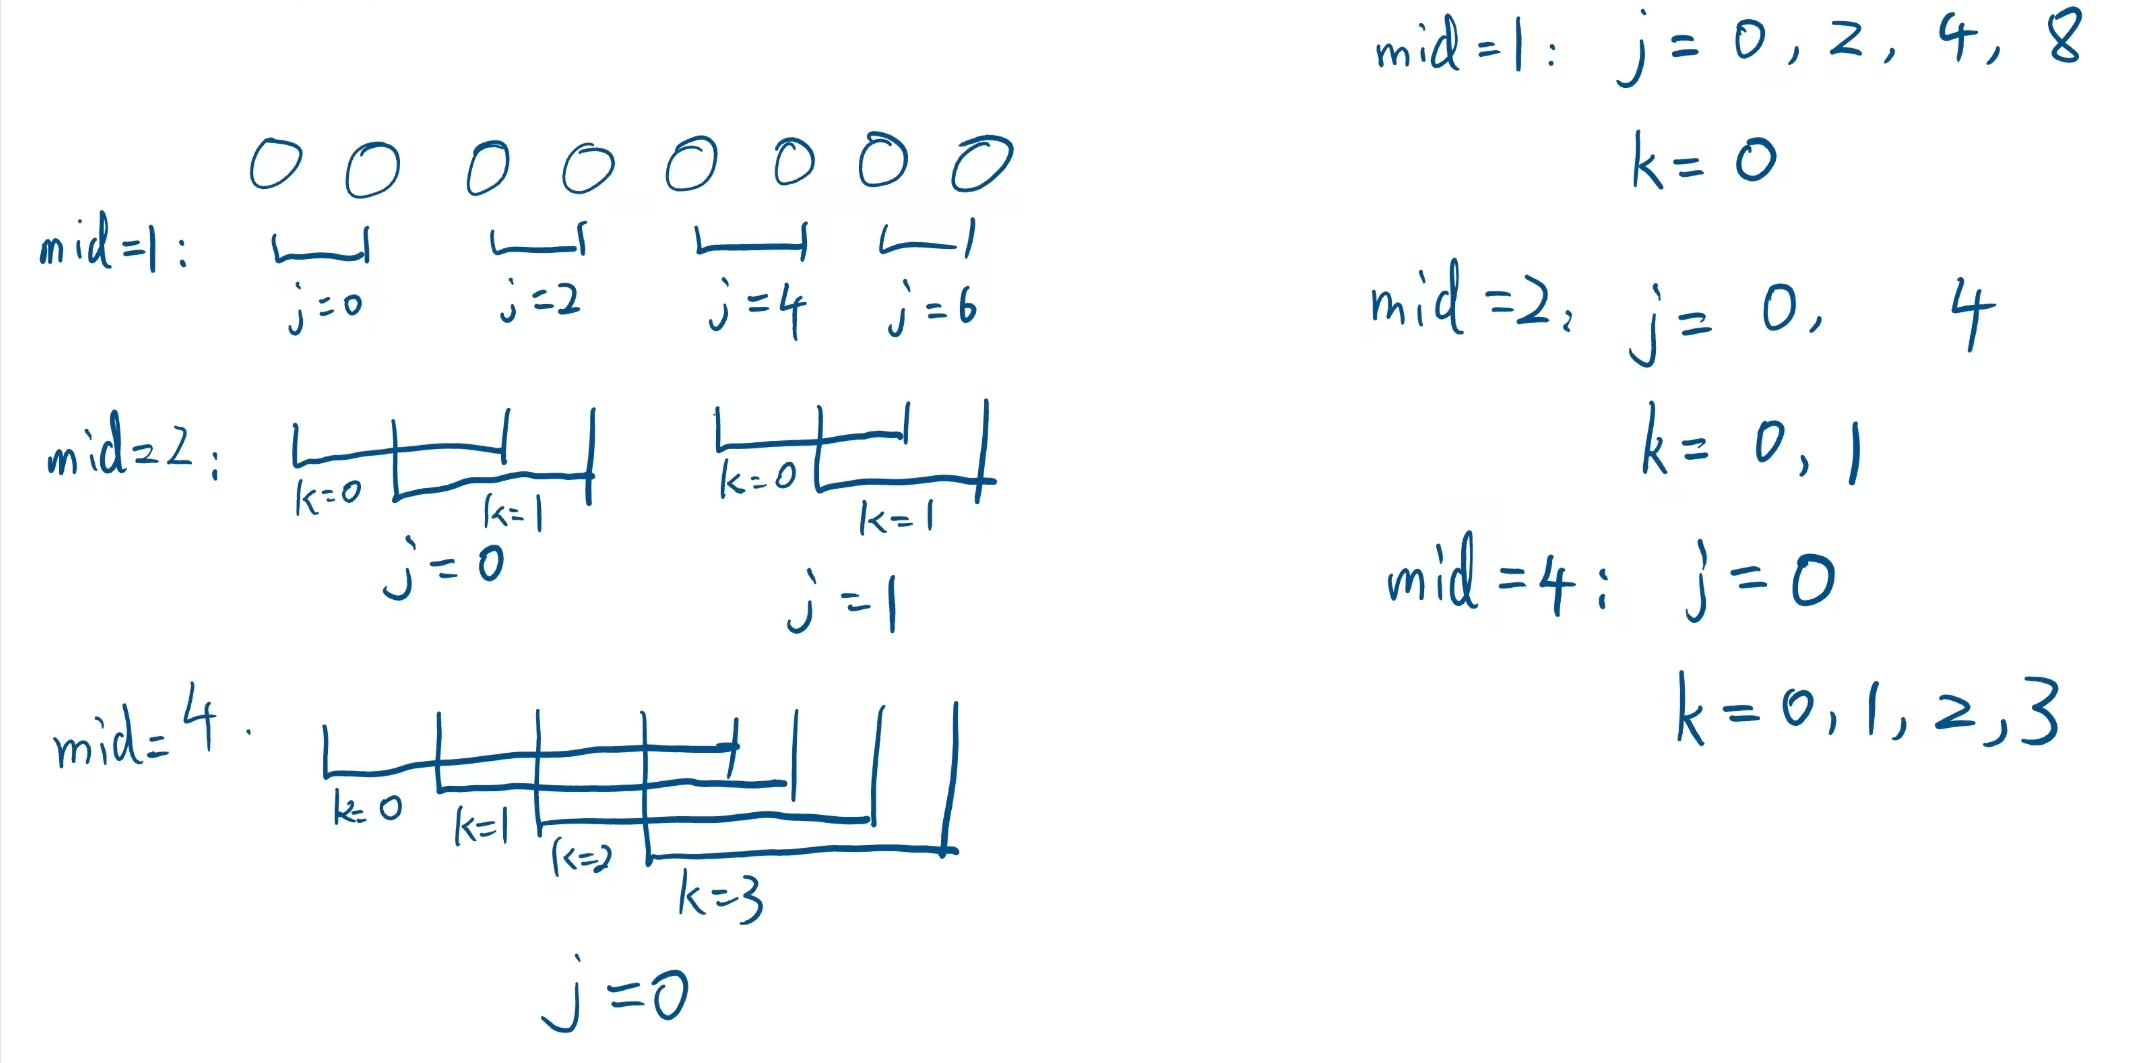
\includegraphics[width=0.8\textwidth]{image/1.png}
    \caption{蝶形运算变量行为}
    \label{p2}
\end{figure}

我们可以看到,\texttt{mid}始终为 2 的幂次(废话)。当\texttt{mid}为 1 或 2 时,蝶形运算均在单个\texttt{u32x4}向量内部进行;只有在\texttt{mid}大于等于 4 的时候,蝶形运算才能在两个\texttt{u32x4}之间进行。

因此,要把它整理成便于并行化的形式,我们需要针对\texttt{mid}进行分类讨论。

\subsection{当\texttt{mid}等于 1 时}

当\texttt{mid}等于 1 时,k 只能是 0,因此可以简单直接地消除循环:

\begin{lstlisting}[language=C++]
case 1:
{
  for (u32 j = 0; j < n; j += (mid << 1))
  {
    u32_mont w_mont = montMod.from_u32(1);
    u32_mont x_mont = a_mont[j];
    u32_mont y_mont = montMod.mul(w_mont, a_mont[j + 1]);
    a_mont[j] = montMod.add(x_mont, y_mont);
    a_mont[j + 1] = montMod.sub(x_mont, y_mont);
  }
  break;
}
\end{lstlisting}

\subsection{当\texttt{mid}等于 2 时}

当\texttt{mid}等于 2 时,k 可以是 0 或 1,因此消除循环后还需要对代码逻辑进行一次复制。

另外,需要额外注意的是第三层\texttt{for}循环里对\texttt{w\_mont}的变换。在消除\texttt{for}循环之后,我们需要手动来计算一次\texttt{w\_mont}。

\begin{lstlisting}[language=C++]
case 2:
{
  u32_mont Wn_mont = montMod.pow(omega_mont, (p - 1) / (mid << 1));
  for (u32 j = 0; j < n; j += (mid << 1))
  {
    u32_mont w_mont_0 = montMod.from_u32(1);
    u32_mont w_mont_1 = montMod.mul(w_mont_0, Wn_mont);
    u32_mont x_mont_0 = a_mont[j + 0];
    u32_mont x_mont_1 = a_mont[j + 1];
    u32_mont y_mont_0 = montMod.mul(w_mont_0, a_mont[j + 2]);
    u32_mont y_mont_1 = montMod.mul(w_mont_1, a_mont[j + 3]);
    a_mont[j + 0] = montMod.add(x_mont_0, y_mont_0);
    a_mont[j + 1] = montMod.add(x_mont_1, y_mont_1);
    a_mont[j + 2] = montMod.sub(x_mont_0, y_mont_0);
    a_mont[j + 3] = montMod.sub(x_mont_1, y_mont_1);
  }
  break;
}
\end{lstlisting}

\subsection{当\texttt{mid}至少为 4 时}

当\texttt{mid}至少为 4 时,我们便可以充分利用 SIMD 指令进行并行化计算。此时,我们可以一次处理 4 个连续的元素,因为:

\begin{enumerate}
    \item \texttt{a[j+k]}到\texttt{a[j+k+3]}是连续的 4 个元素,可以被打包成一个 SIMD 向量
    \item \texttt{a[j+k+mid]}到\texttt{a[j+k+mid+3]}也是连续的 4 个元素,同样可以被打包成一个 SIMD 向量
    \item 旋转因子\texttt{w\_mont\_0}到\texttt{w\_mont\_3}也可以被打包成一个 SIMD 向量
\end{enumerate}

在串行代码中,我们展开循环,手动计算四个连续的旋转因子和相应的运算:

\begin{lstlisting}[language=C++]
default: // mid >= 4, parallelizable
{
  u32_mont Wn_mont = montMod.pow(omega_mont, (p - 1) / (mid << 1));
  for (u32 j = 0; j < n; j += (mid << 1))
  {
    u32_mont w_mont_0 = montMod.from_u32(1);
    u32_mont w_mont_1 = montMod.mul(w_mont_0, Wn_mont);
    u32_mont w_mont_2 = montMod.mul(w_mont_1, Wn_mont);
    u32_mont w_mont_3 = montMod.mul(w_mont_2, Wn_mont);
    u32_mont Wn_mont_4 = montMod.pow(Wn_mont, 4);
    for (u32 k = 0; k < mid; k += 4)
    {
      u32_mont x_mont_0 = a_mont[j + k + 0];
      u32_mont x_mont_1 = a_mont[j + k + 1];
      u32_mont x_mont_2 = a_mont[j + k + 2];
      u32_mont x_mont_3 = a_mont[j + k + 3];

      u32_mont y_mont_0 = montMod.mul(w_mont_0, a_mont[j + k + mid + 0]);
      u32_mont y_mont_1 = montMod.mul(w_mont_1, a_mont[j + k + mid + 1]);
      u32_mont y_mont_2 = montMod.mul(w_mont_2, a_mont[j + k + mid + 2]);
      u32_mont y_mont_3 = montMod.mul(w_mont_3, a_mont[j + k + mid + 3]);

      a_mont[j + k + 0] = montMod.add(x_mont_0, y_mont_0);
      a_mont[j + k + 1] = montMod.add(x_mont_1, y_mont_1);
      a_mont[j + k + 2] = montMod.add(x_mont_2, y_mont_2);
      a_mont[j + k + 3] = montMod.add(x_mont_3, y_mont_3);

      a_mont[j + k + mid + 0] = montMod.sub(x_mont_0, y_mont_0);
      a_mont[j + k + mid + 1] = montMod.sub(x_mont_1, y_mont_1);
      a_mont[j + k + mid + 2] = montMod.sub(x_mont_2, y_mont_2);
      a_mont[j + k + mid + 3] = montMod.sub(x_mont_3, y_mont_3);

      w_mont_0 = montMod.mul(w_mont_0, Wn_mont_4);
      w_mont_1 = montMod.mul(w_mont_1, Wn_mont_4);
      w_mont_2 = montMod.mul(w_mont_2, Wn_mont_4);
      w_mont_3 = montMod.mul(w_mont_3, Wn_mont_4);
    }
  }
  break;
}
\end{lstlisting}

\section{封装基本并行运算}\label{sec:parallel_ops}

为了简化主要逻辑、避免呈现过多并行化的 Montgomery 规约模运算细节,同时也为了使并行化的过程更直观,我们实现了\texttt{MontModNeon}类,将需要用到的并行运算封装起来。下面简要讲解其实现:

\subsection{基本结构与成员变量}

\begin{lstlisting}[language=C++]
class MontModNeon
{
private:
    u32 mod;       // 模数
    u32 r2;        // r^2 mod mod
    u32 neg_r_inv; // -r^(-1) mod 2^32

    u32x4 mod_vec;       // 向量化的模数
    u32x4 neg_r_inv_vec; // 向量化的 -r^(-1) mod 2^32
};
\end{lstlisting}

核心成员变量包括模数\texttt{mod}、r 的平方\texttt{r2}、负模逆元\texttt{neg\_r\_inv},以及它们的向量化表示\texttt{mod\_vec}和\texttt{neg\_r\_inv\_vec}。

\subsection{数据类型转换}

\begin{lstlisting}[language=C++]
u32x4_mont from_u32x4(u32x4 a) const
{
    u64x2 t0 = vmull_u32(vget_low_u32(a), vdup_n_u32(r2));
    u64x2 t1 = vmull_u32(vget_high_u32(a), vdup_n_u32(r2));
    return reduce_pair(t0, t1);
}

u32x4 to_u32x4(u32x4_mont a_mont) const { return reduce(a_mont); }
\end{lstlisting}

这两个函数实现了普通向量和 Montgomery 域向量之间的转换。\texttt{from\_u32x4}将普通向量转换为 Montgomery 域,需要将每个元素乘以 r² 然后进行规约;\texttt{to\_u32x4}则执行相反的操作。

\subsection{Montgomery 规约}

\begin{lstlisting}[language=C++]
u32x4_mont reduce(u32x4 t_lo) const
{
    // t_lo 是低32位,高32位补0,提升成64位
    u64x2 t0 = vmovl_u32(vget_low_u32(t_lo));
    u64x2 t1 = vmovl_u32(vget_high_u32(t_lo));

    return reduce_pair(t0, t1);
}

u32x4_mont reduce_pair(u64x2 t0, u64x2 t1) const
{
    // m = (t mod 2^32) * neg_r_inv mod 2^32
    u32x2 m0 = vmul_u32(vmovn_u64(t0), vget_low_u32(neg_r_inv_vec));
    u32x2 m1 = vmul_u32(vmovn_u64(t1), vget_high_u32(neg_r_inv_vec));

    // t + m * mod
    u64x2 t0_new = vmlal_u32(t0, m0, vget_low_u32(mod_vec));
    u64x2 t1_new = vmlal_u32(t1, m1, vget_high_u32(mod_vec));

    // (t + m * mod) >> 32
    u32x2 res0 = vshrn_n_u64(t0_new, 32);
    u32x2 res1 = vshrn_n_u64(t1_new, 32);

    u32x4 res = vcombine_u32(res0, res1);

    // res = res - (mod & -(res >= mod))
    uint32x4_t mask = vcgeq_u32(res, mod_vec); // res >= mod
    uint32x4_t mod_masked = vandq_u32(mod_vec, mask);
    res = vsubq_u32(res, mod_masked);

    return res;
}
\end{lstlisting}

这是类中最核心的部分,实现了向量化的 Montgomery 规约。该操作将一个 64 位长整数(或两个 32 位整数的乘积)转换为其在 Montgomery 域中的表示。函数使用 NEON 指令完成以下步骤:

\begin{enumerate}
    \item 计算 m = (t mod 2\^{}32) * neg\_r\_inv mod 2\^{}32
    \item 计算 t + m * mod
    \item 将结果右移 32 位
    \item 如果结果大于等于 mod,则减去 mod
\end{enumerate}

这样,我们避免了直接的除法运算,而是通过乘法、加法和位移操作完成了模运算。

\subsection{基本运算函数}

\begin{lstlisting}[language=C++]
u32x4_mont add(u32x4_mont a, u32x4_mont b) const
{
    u32x4 res = vaddq_u32(a, b);
    uint32x4_t mask = vcgeq_u32(res, mod_vec);
    uint32x4_t mod_masked = vandq_u32(mod_vec, mask);
    return vsubq_u32(res, mod_masked);
}

u32x4_mont sub(u32x4_mont a, u32x4_mont b) const
{
    uint32x4_t mask = vcgeq_u32(a, b);
    u32x4 res1 = vsubq_u32(a, b);
    u32x4 res2 = vsubq_u32(vaddq_u32(a, mod_vec), b);
    return vbslq_u32(mask, res1, res2);
}

u32x4_mont mul(u32x4_mont a, u32x4_mont b) const
{
    u64x2 prod0 = vmull_u32(vget_low_u32(a), vget_low_u32(b));
    u64x2 prod1 = vmull_u32(vget_high_u32(a), vget_high_u32(b));
    return reduce_pair(prod0, prod1);
}
\end{lstlisting}

这些函数实现了向量化的基本算术运算:

\begin{itemize}
    \item \texttt{add}:向量化的模加法,先执行加法,再根据是否溢出执行条件减法
    \item \texttt{sub}:向量化的模减法,根据大小关系选择直接减法或先加模数再减法
    \item \texttt{mul}:向量化的模乘法,将 32 位乘法扩展为 64 位,然后进行 Montgomery 规约
\end{itemize}

此外,类中还实现了向量化的模幂和模逆元计算:

\begin{lstlisting}[language=C++]
u32x4_mont pow(u32x4_mont base_mont, u32 exp) const
{
    u32x4 result_mont = from_u32x4(vdupq_n_u32(1));
    while (exp > 0)
    {
        if (exp & 1)
            result_mont = mul(result_mont, base_mont);
        base_mont = mul(base_mont, base_mont);
        exp >>= 1;
    }
    return result_mont;
}

u32x4_mont inv(u32x4_mont x_mont) const { return pow(x_mont, mod - 2); }
\end{lstlisting}

\section{并行化代码}

并行化的主要任务有二:其一是基于前述铺垫,对便于并行化的串行前向与逆向 NTT 进行并行化;其二是修改多项式乘法的函数,使其使用向量化的\texttt{a\_simd[]}代替标量化的\texttt{a[]}参与运算即可。

\subsection{并行化前向与逆向 NTT}

经过了前面的铺垫,这一步反而是最简单的:只需要把\texttt{switch}块中的\texttt{defalut}部分中的所有四个一组的标量整合为一个向量进行运算即可。除此以外,我们还需要针对\texttt{mid}等于\texttt{1}和\texttt{2}这两种情况下的标量运算进行标量向量转换。

由于前向和逆向两个变换在结构上的高度相似,此处,我们仅就前向 NTT 变换\texttt{ntt\_forward\_mont\_simd}进行介绍。

\subsubsection{向量化蝶形运算}

对于\texttt{mid >= 4}的情况,将标量运算替换为向量化运算。例如:

\begin{lstlisting}[language=C++]
// 标量版本
x_mont_0 = a_mont[j+k+0];
x_mont_1 = a_mont[j+k+1];
x_mont_2 = a_mont[j+k+2];
x_mont_3 = a_mont[j+k+3];

y_mont_0 = montMod.mul(w_mont_0,
           a_mont[j+k+mid+0]);
\end{lstlisting}

被替换为

\begin{lstlisting}[language=C++]
// 向量化版本
x_monts_simd = a_mont_simd[(j+k)/4];

y_monts_simd = montModNeon.mul(
  w_monts_simd, a_mont_simd[(j+k+mid)/4]);
\end{lstlisting}

相同的替换模式也应用于加减运算和旋转因子更新:

\begin{lstlisting}[language=C++]
a_mont_simd[(j+k)/4] = montModNeon.add(x_monts_simd, y_monts_simd);
a_mont_simd[(j+k+mid)/4] = montModNeon.sub(x_monts_simd, y_monts_simd);
w_monts_simd = montModNeon.mul(w_monts_simd, Wn_mont_4_simd);
\end{lstlisting}

\subsubsection{标量/向量运算状态管理}

函数使用一个\texttt{is\_serial}布尔变量来跟踪当前数据是处于标量形式还是向量形式,根据需要进行转换:

\begin{lstlisting}[language=C++]
bool is_serial = false;  // 默认认为数据是向量形式
u32_mont *a_mont = new u32_mont[n];  // 用于标量计算的缓冲区
\end{lstlisting}

每当遇到需要切换计算模式时,会进行相应的转换:

\begin{lstlisting}[language=C++]
// 从向量形式转为标量形式
if (!is_serial)
{
    from_simd(a_mont, a_mont_simd, n);
    is_serial = true;
}

// 从标量形式转为向量形式
if (is_serial)
{
    to_simd(a_mont, a_mont_simd, n);
    is_serial = false;
}
\end{lstlisting}

在\texttt{mid = 1}时,我们转换到标量形式进行运算;在\texttt{mid >= 4}时,我们转换到向量形式进行运算;在函数结束时,我们通过\texttt{is\_serial}判断是否应当将数据转回向量形式,以便后续处理:

\subsection{并行化多项式乘法}

最后,我们基于并行化的 NTT 实现多项式乘法函数。由于大部分逻辑与原本的并无差别,这里我们重点分析向量化与去向量化的时机,解释我们为什么在比特翻转之后、在转换到 Montgomery 域之前进行向量化;去向量化的过程与向量化正好相反,此处亦不做赘述。

\subsubsection{在比特翻转之后向量化}

显然,比特翻转操作的不连续性会导致向量内部的数据被大量修改。如果要对比特翻转操作进行并行化,势必会引入大量的向量包装与解包操作,这会降低效率,而且实现起来很麻烦,得不偿失。

因此,我们把向量化放在比特翻转之后进行,让多项式系数在标量状态下进行比特翻转之后,才进行向量化。

\subsubsection{在转换到 Montgomery 域之前向量化}

其实这也是挺显然的,Montgomery 转换本身便是 SIMD 的,内存连续,适合并行化。因此我们在转换到 Montgomery 域之前向量化。

\section{性能分析}

在本次实验中,我们对 NTT 算法实现了多个版本的优化,包括基础串行实现(naive)、NTT 优化的串行实现(serial)、Montgomery 规约优化(montgomery)以及 SIMD 并行优化(parallel)。下面我们将分析不同版本在不同多项式长度下的性能表现。随后,我们将重点就 SIMD 并行优化的代码,使用 perf 进行深入的性能测试与剖析。

\subsection{各版本的测试结果}

我们在在校方服务器环境下,对各个版本的算法进行测试,记录不同规模下的平均延迟(单位:微秒),如表\ref{t1}所示。同时,我们将结果在对数坐标下绘制为图表\ref{p1},以便直观地对比各个版本在不同数据规模下的平均延迟。

\begin{table}[h]
\centering
\begin{tabular}{|l|c|c|c|}
\hline
实现版本 & n=4 & n=131072 & 对大规模的加速比 \\ \hline
基础串行(naive) & 0.00018 & 95420.7 & 1.0$\times$ \\ \hline
优化串行(serial) & 0.0041 & 104.736 & 910.9$\times$ \\ \hline
Montgomery(montgomery) & 0.00485 & 76.1702 & 1252.7$\times$ \\ \hline
SIMD 并行(parallel) & 0.01747 & 65.9827 & 1446.1$\times$ \\ \hline
\end{tabular}
\caption{不同实现在不同规模下的性能对比}
\label{t1}
\end{table}

\begin{figure}[h]
    \centering
    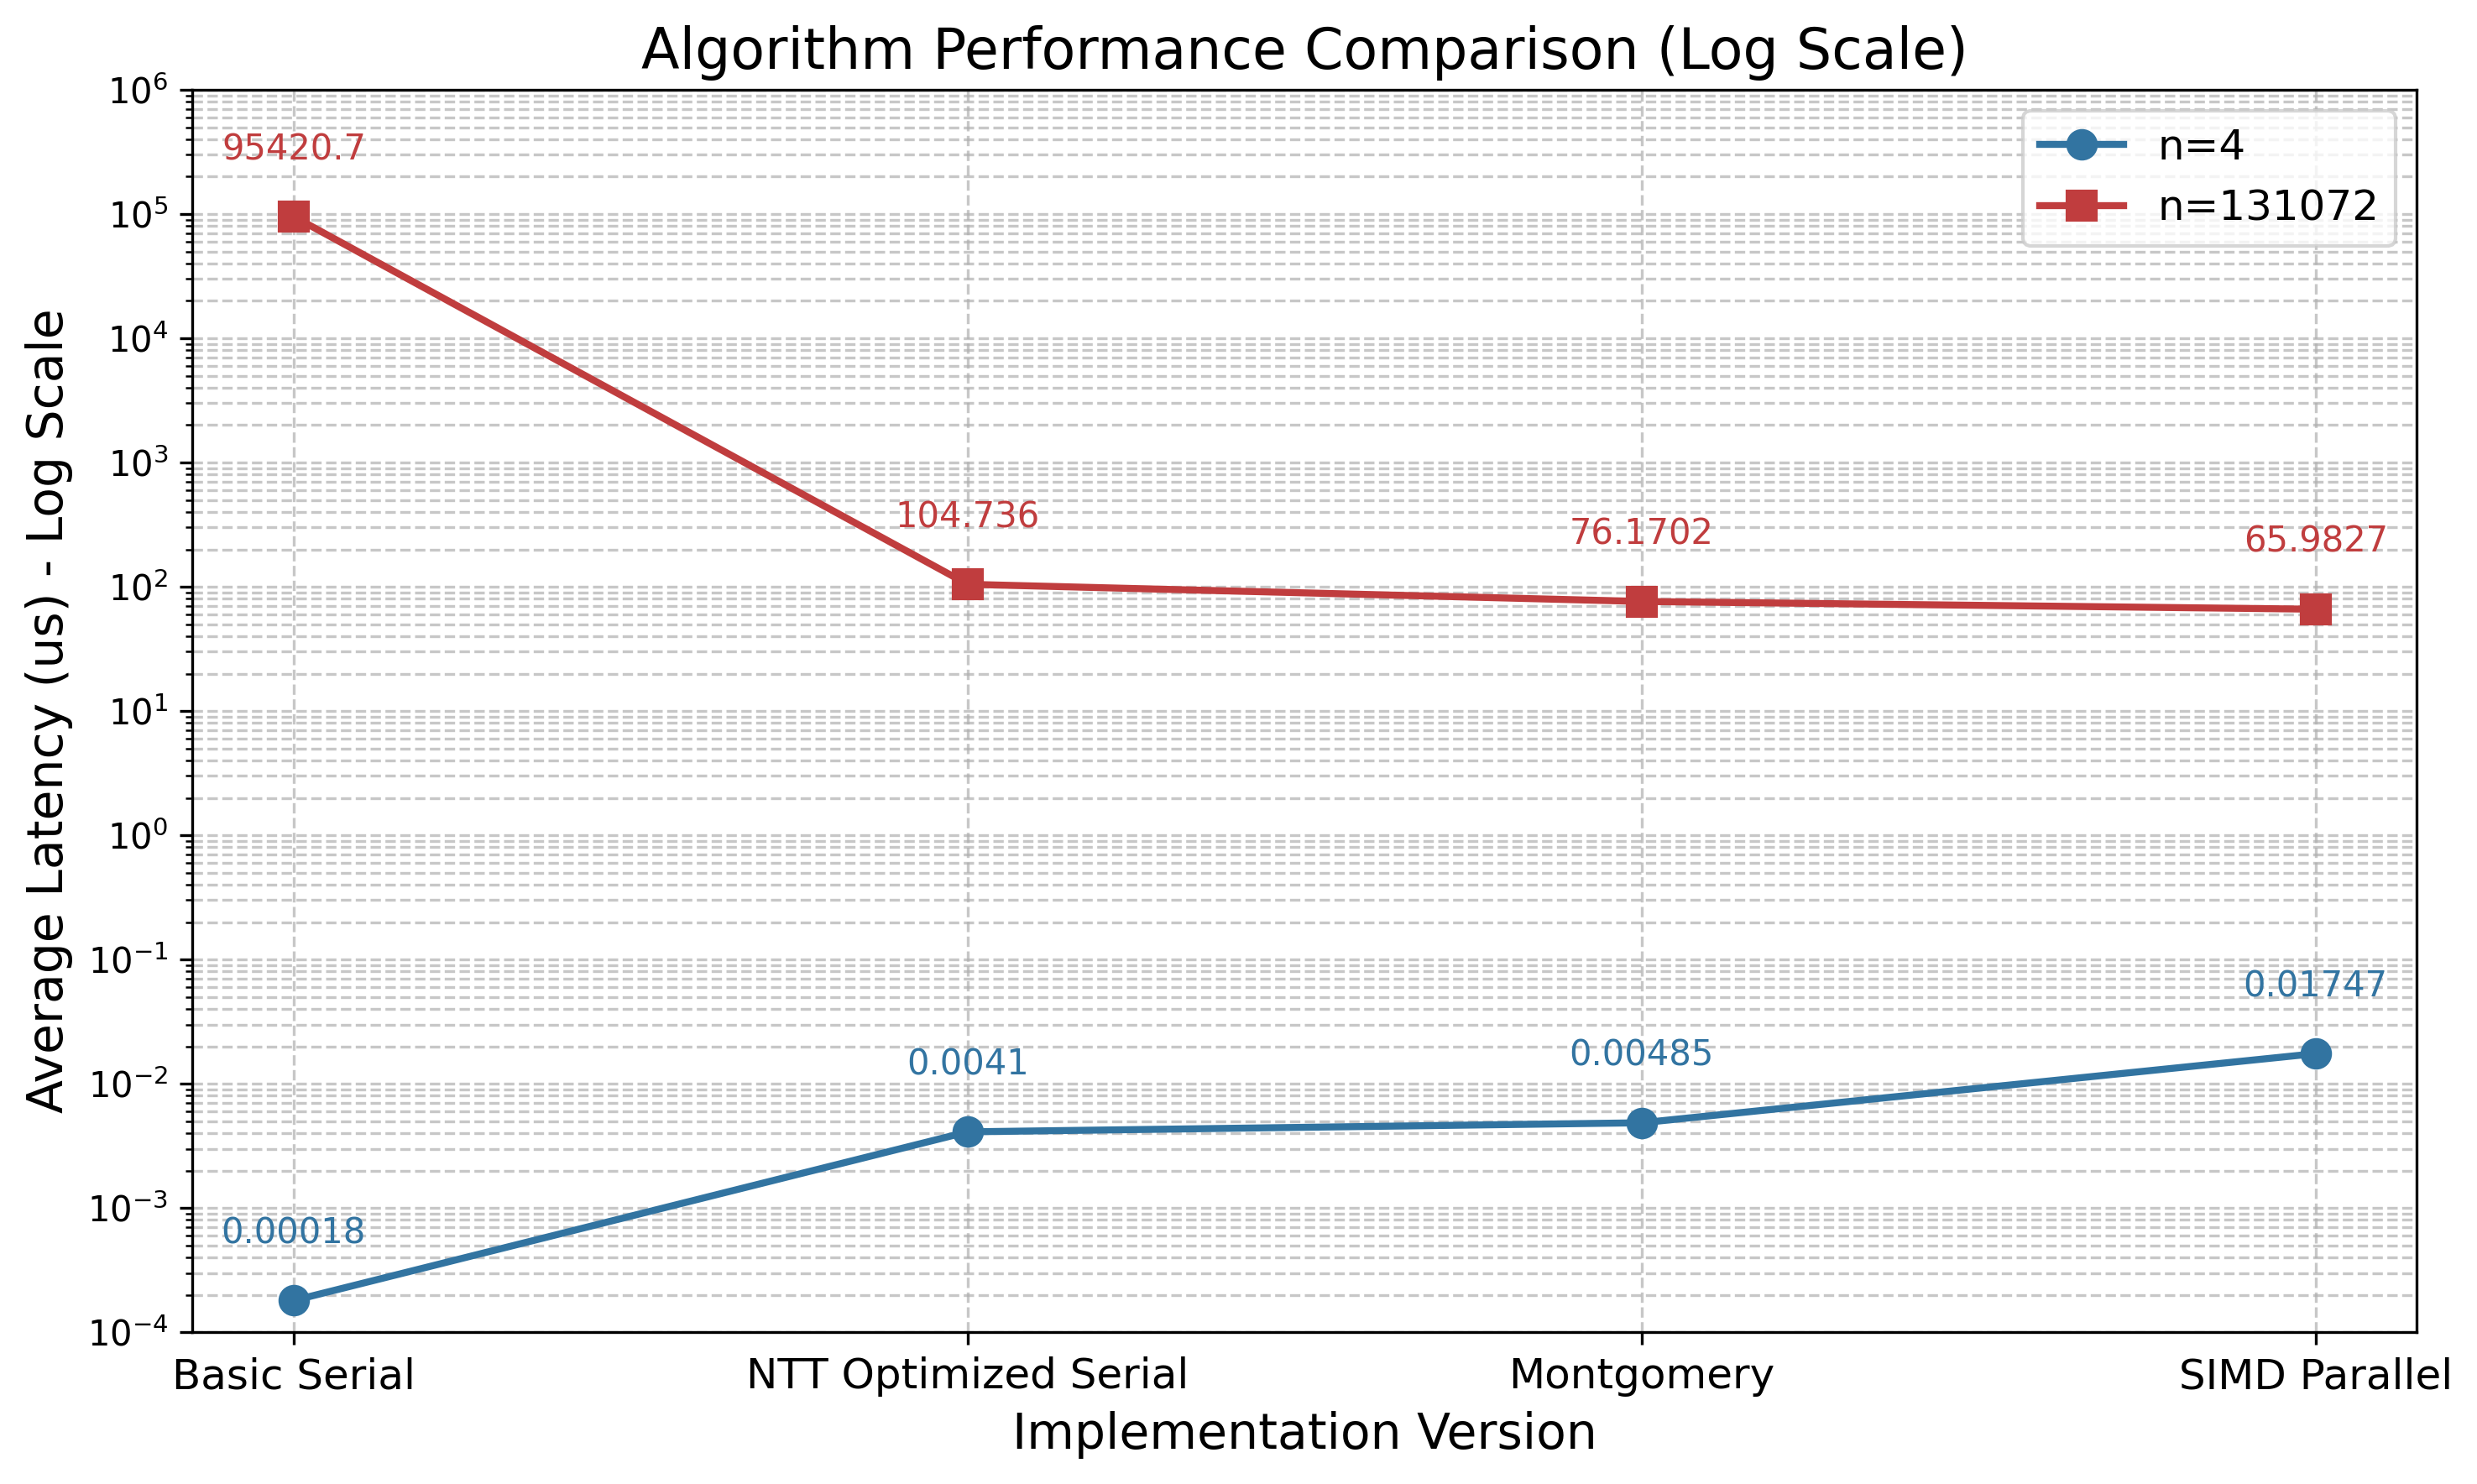
\includegraphics[width=0.8\textwidth]{image/2.png}
    \caption{各版本在不同数据规模下的平均延迟对比(对数坐标)}
    \label{\p1}
\end{figure}

我们可以发现,在小规模数据(n=4)下,基础串行版本反而表现出最低的延迟。我们认为,这是因为优化版本引入的额外开销(如初始化 Montgomery 常量、SIMD 向量的包装与解包等)在小数据量下无法抵消获得的收益;甚至,在\texttt{n = 4}的极小规模下,我们的代码完全无法进行 SIMD 运算,反而由于向量化和去向量化的操作引入了大量的无用操作。

除此以外,在大规模数据(n=131072)下,各个优化版本都展现出显著的性能优势:优化串行版本相比基础串行版本提升了约 910 倍,这一巨大提升主要来自于算法结构的优化,直接将复杂度从$O(n^2)$降为$O(n\cdot log(n))$。Montgomery 规约优化进一步将性能提升了约 27\%,SIMD 并行优化使性能又提升了约 13\%,虽然提升幅度不及前两次优化大,但在已经高度优化的代码基础上实现这样的提升仍然很有价值。

\subsection{使用 perf 进行深入剖析}

我们使用 perf 记录我们的并行优化代码对长为 32768 的多项式进行乘法运算的过程,并使用 perf 的 report 工具查看结果。表\ref{t2}记录了部分摘录与分析,也可参照火焰图\ref{fig:enter-label}.

\begin{table}[h]
\centering
\begin{tabular}{|l|l|l|l|}
\hline
Children & Self & Symbol & 分析与注释 \\ \hline
99.64\% & 0.00\% & \texttt{\_start} $\rightarrow$ \texttt{\_\_libc\_start\_main} $\rightarrow$ \texttt{main} & 主程序(包括随机测试样例生成) \\ \hline
89.13\% & 0.36\% & \texttt{poly\_multiply\_ntt\_simd} & 多项式乘法 \\ \hline
47.64\% & 1.81\% & \texttt{ntt\_forward\_mont\_simd} & 正向 NTT \\ \hline
42.93\% & \textbf{42.93\%} & \texttt{MontModNeon::reduce\_pair} & 热点之一:Montgomery reduction 双输入版 \\ \hline
25.36\% & 0.91\% & \texttt{ntt\_inverse\_mont\_simd} & 逆向 NTT \\ \hline
24.46\% & \textbf{24.46\%} & \texttt{MontModNeon::mul} & 热点之二:SIMD 版的模乘 \\ \hline
8.51\% & 8.51\% & \texttt{bit\_reverse\_permute} & 位反转置换 \\ \hline
5.43\% & 5.43\% & \texttt{MontMod::reduce} & 标准版的 Montgomery reduction \\ \hline
5.07\% & 5.07\% & \texttt{MontModNeon::sub} & SIMD 的模减 \\ \hline
3.99\% & 3.99\% & \texttt{MontModNeon::add} & SIMD 的模加 \\ \hline
\end{tabular}
\caption{perf 分析结果}
\label{t2}
\end{table}

\begin{figure}
    \centering
    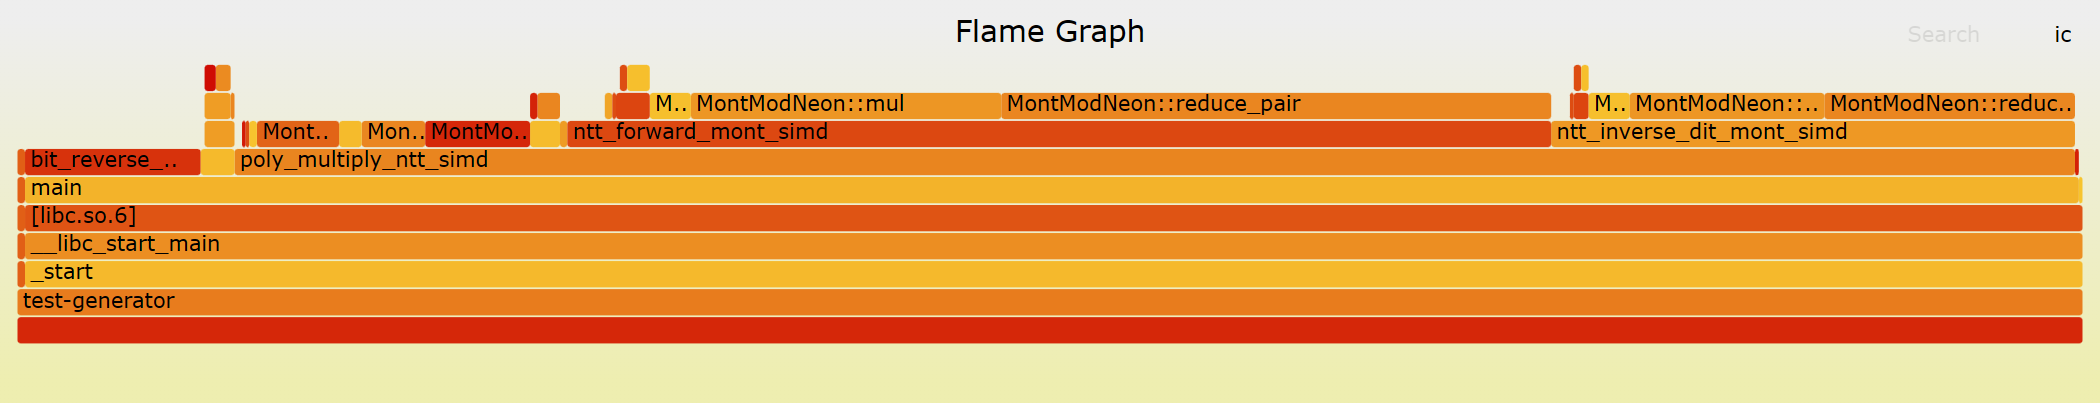
\includegraphics[width=1\linewidth]{image/3.png}
    \caption{perf 分析结果的火焰图表示}
    \label{fig:enter-label}
\end{figure}

可以看到,\texttt{MontModNeon::reduce\_pair}和\texttt{MontModNeon::mul}所占用的运行时间是最多的。

我们不难理解\texttt{MontModNeon::mul}占用时间较长(因为多项式乘法本身便会用到大量的乘法)。事实上,由于\texttt{MontModNeon::mul}会调用\texttt{MontModNeon::reduce\_pair},后者占用时间较长也不难理解。

下面我们分析\texttt{MontModNeon::reduce\_pair}占用时间长的原因:

\subsubsection{逻辑复杂度}

在 \texttt{reduce\_pair} 里,实际执行的操作很多:

\begin{itemize}
    \item \texttt{vmovn\_u64}:64 位降到 32 位
    \item \texttt{vmul\_u32}:乘法
    \item \texttt{vmlal\_u32}:64 位加乘(multiply-accumulate)
    \item \texttt{vshrn\_n\_u64}:右移
    \item \texttt{vcgeq\_u32}:比较
    \item \texttt{vandq\_u32}:按位与
    \item \texttt{vsubq\_u32}:减法
\end{itemize}

不仅如此,其中,\texttt{vmlal\_u32}和\texttt{vshrn\_n\_u64}耗时都较长。

另一方面,\texttt{vcgeq\_u32}、\texttt{vandq\_u32}和\texttt{vsubq\_u32}构成逻辑判断,使依赖关系变得复杂,产生了内部数据依赖,导致流水线阻塞。

\subsubsection{内部数据依赖导致流水线阻塞}

从指令链看,\texttt{reduce\_pair}是顺序依赖非常密集的:

\begin{itemize}
    \item 要先 \texttt{vmovn}(截断低 32 位),才能 \texttt{vmul}(乘 neg\_r\_inv)
    \item 要 \texttt{vmlal}(t + m$\times$mod),然后才能 \texttt{vshrn}(右移)
    \item 要 \texttt{vshrn} 之后才能做比较、条件修正
\end{itemize}

因为没有办法把这些阶段并行展开,所以 CPU 在执行这段的时候,流水线容易空转等待。

\subsubsection{结论}

\texttt{MontModNeon::reduce\_pair} 之所以占用这么多时间,既有逻辑复杂度高的原因,也有数据强依赖导致的流水线阻塞的原因。

由于这里的各个操作无法化简,要想进一步提升程序效率,我们可以从流水线重排的角度解决流水线阻塞的问题。不过这就超出我们 SIMD 实验的范畴了,我们在此不做进一步优化。

\end{document}
